% ===================== Section III: Dataset (Member 1) =====================
\section{Dataset}
\label{sec:dataset}

\subsection{Source and Licence}

We use the Base dataset of the Bank Account Fraud (BAF) suite \cite{jesus2022turning}, which is
available on Kaggle and GitHub \cite{baf2022kaggle} under the CC BY-NC-ND 4.0 licence, so it may be
used for non-commercial research without changes to the data itself. The suite was created by Feedzai
from a real, anonymised dataset of online bank account applications at a large consumer bank. Each
row is a synthetic application produced by a CTGAN generative model, and noise was added to give a
degree of differential privacy, so no row belongs to a real person \cite{jesus2022turning}. The
fraud labels in the original data were collected several months after the accounts were opened.
The suite contains six datasets of one million rows each; the Base dataset keeps the natural biases
of the original data, while the five variants add controlled types of bias. We use only the Base
dataset, as required by the topic.

\subsection{Size and Features}

The Base dataset has \tbd{1,000,000} applications and \tbd{32} columns: the label
\texttt{fraud\_bool}, the application \texttt{month} (0 to 7), and 30 features. Five features are
categorical with anonymised levels (\texttt{payment\_type}, \texttt{employment\_status},
\texttt{housing\_status}, \texttt{source}, \texttt{device\_os}); the rest are numeric or binary.
The data contains three attributes that are treated as protected in the BAF paper: age
(\texttt{customer\_age}, rounded to the decade), income (\texttt{income}, in deciles) and
employment status. For the description and for the ablation study we group the features into six
groups by what they describe (Table~\ref{tab:groups}). The application velocity group holds
aggregated counts, such as the number of applications per hour in the last 6 hours, 24 hours and 4
weeks, or the number of applications from the same zip code in the last 4 weeks.

\begin{table}[!t]
\centering
\caption{Feature groups used in the dataset description and the ablation study.}
\label{tab:groups}
\footnotesize
\setlength{\tabcolsep}{3.5pt}
\begin{tabular}{>{\raggedright\arraybackslash}p{1.55cm}>{\raggedright\arraybackslash}p{6.3cm}}
\hline
Group & Features \\
\hline
Applicant (4) & \texttt{\footnotesize income}, \texttt{\footnotesize customer\_\allowbreak age}, \texttt{\footnotesize employment\_\allowbreak status}, \texttt{\footnotesize housing\_\allowbreak status} \\
Address history (2) & \texttt{\footnotesize prev\_\allowbreak address\_\allowbreak months\_\allowbreak count}, \texttt{\footnotesize current\_\allowbreak address\_\allowbreak months\_\allowbreak count} \\
Email and phone (4) & \texttt{\footnotesize name\_\allowbreak email\_\allowbreak similarity}, \texttt{\footnotesize email\_\allowbreak is\_\allowbreak free}, \texttt{\footnotesize phone\_\allowbreak home\_\allowbreak valid}, \texttt{\footnotesize phone\_\allowbreak mobile\_\allowbreak valid} \\
Application velocity (7) & \texttt{\footnotesize velocity\_\allowbreak 6h}, \texttt{\footnotesize velocity\_\allowbreak 24h}, \texttt{\footnotesize velocity\_\allowbreak 4w}, \texttt{\footnotesize zip\_\allowbreak count\_\allowbreak 4w}, \texttt{\footnotesize bank\_\allowbreak branch\_\allowbreak count\_\allowbreak 8w}, \texttt{\footnotesize date\_\allowbreak of\_\allowbreak birth\_\allowbreak distinct\_\allowbreak emails\_\allowbreak 4w}, \texttt{\footnotesize days\_\allowbreak since\_\allowbreak request} \\
Credit and banking (6) & \texttt{\footnotesize credit\_\allowbreak risk\_\allowbreak score}, \texttt{\footnotesize proposed\_\allowbreak credit\_\allowbreak limit}, \texttt{\footnotesize intended\_\allowbreak balcon\_\allowbreak amount}, \texttt{\footnotesize payment\_\allowbreak type}, \texttt{\footnotesize bank\_\allowbreak months\_\allowbreak count}, \texttt{\footnotesize has\_\allowbreak other\_\allowbreak cards} \\
Device and session (6) & \texttt{\footnotesize device\_\allowbreak os}, \texttt{\footnotesize source}, \texttt{\footnotesize session\_\allowbreak length\_\allowbreak in\_\allowbreak minutes}, \texttt{\footnotesize keep\_\allowbreak alive\_\allowbreak session}, \texttt{\footnotesize device\_\allowbreak distinct\_\allowbreak emails\_\allowbreak 8w}, \texttt{\footnotesize foreign\_\allowbreak request} \\
\hline
\end{tabular}
\end{table}


\subsection{Class Balance and Time}

Only \tbd{11,029} applications (\tbd{1.10\%}) are fraudulent. Fig.~\ref{fig:months} shows the
number of applications and the fraud rate in each month. \tbd{Describe: months differ in size from
X to Y applications; fraud rate ranges from A\% (month M) to B\% (month N); the test months have a
higher/lower rate than the development months.} This means that the prior probability of fraud
itself moves over time, which is one of the reasons why a threshold chosen on earlier months may
not give the same false positive rate later.

\begin{figure}[!t]
\centering
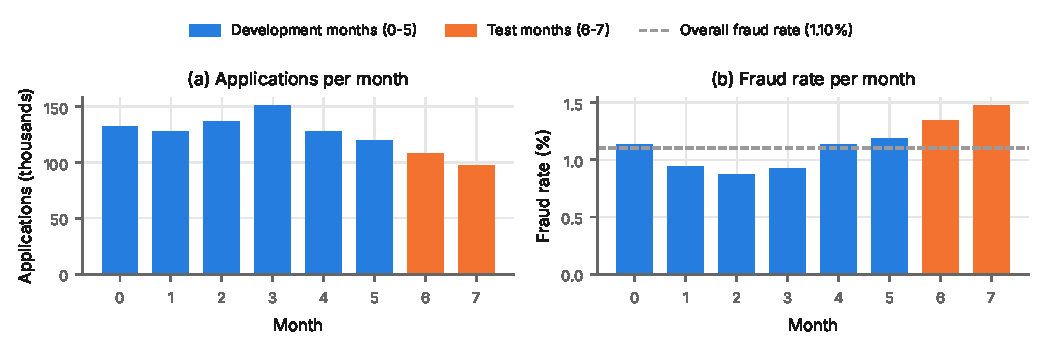
\includegraphics[width=\columnwidth]{figures/eda_months.pdf}
\caption{Applications (a) and fraud rate (b) per month in the BAF Base dataset. Months 0--5 (blue)
are used for development and months 6--7 (orange) for testing; the dashed line is the overall fraud
rate.}
\label{fig:months}
\end{figure}

\subsection{Protected Attribute: Age}

Fig.~\ref{fig:age} shows the age distribution and the fraud rate per age decade. \tbd{X\%} of
applicants are in the group older than 50 used in our fairness analysis. Their fraud rate is
\tbd{A\%}, against \tbd{B\%} for applicants aged 50 or under. \tbd{Comment on the trend of fraud
rate with age.} Because the older group has a higher base rate of fraud, a model can learn to rely
on age, which would raise the false positive rate for genuine older applicants. This is what RQ3
measures.

\begin{figure}[!t]
\centering
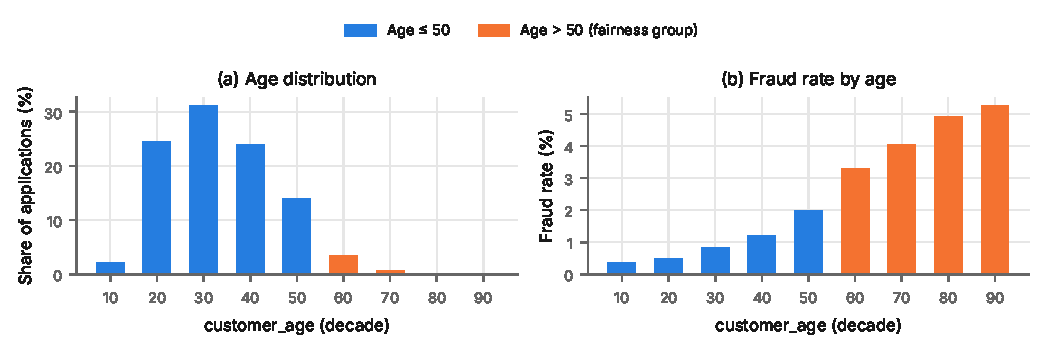
\includegraphics[width=\columnwidth]{figures/eda_age.pdf}
\caption{Share of applications (a) and fraud rate (b) by \texttt{customer\_age} decade. Orange bars
are the group older than 50 used in the fairness analysis.}
\label{fig:age}
\end{figure}

\subsection{Missing Values}

The file has no empty cells, but the datasheet states that in five features a value of $-1$ means
``missing'' and that any negative value of \texttt{intended\_balcon\_amount} is missing
\cite{baf2022kaggle}. After decoding them, \tbd{describe rates: e.g. intended\_balcon\_amount X\%,
prev\_address\_months\_count Y\%, \ldots, session\_length\_in\_minutes Z\%}
(Fig.~\ref{fig:missing}a). Missingness is not random: \tbd{describe which missing values go with
higher/lower fraud rates} (Fig.~\ref{fig:missing}b). For this reason we add a binary
``was missing'' indicator for every such feature instead of only filling the gap.

\begin{figure}[!t]
\centering
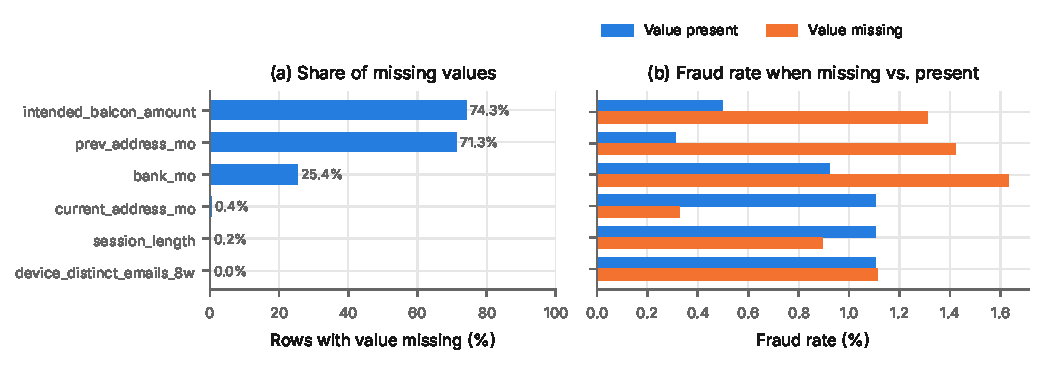
\includegraphics[width=\columnwidth]{figures/eda_missing.pdf}
\caption{(a) Share of applications where each feature is missing after decoding the datasheet's
missing-value codes. (b) Fraud rate when the value is present (blue) and missing (orange).}
\label{fig:missing}
\end{figure}

\subsection{Cleaning and Preprocessing}

We made the following cleaning decisions, all of which are applied before any split and none of
which use the label:
\begin{itemize}
  \item the coded missing values described above are converted to real missing values;
  \item \texttt{device\_fraud\_count} \tbd{takes only the value 0} in the Base file, so it carries
        no information and is removed;
  \item \texttt{month} is used only to define the time-based split and never as a model input,
        because the test months 6 and 7 are values the model would never have seen in training;
  \item \texttt{velocity\_6h} has \tbd{N} negative values; they lie inside the range documented in the
        datasheet and are not described as missing, so we keep them as they are, and negative
        \texttt{credit\_risk\_score} values are valid scores;
  \item \tbd{there are no duplicate rows}, and the categorical features are kept as strings for
        one-hot encoding.
\end{itemize}
This leaves 29 input features. All steps that learn from the data, such as imputation, encoding and
scaling, are fitted later inside each training fold (Section~\ref{sec:method-prep}).
